\chapter{EMS Chatfunktion}
\putz
\section{EMS Chat}
Bei EMS war zu beginn des Projektes eine integrierte Chatfunktion geplant. Ein Promoter sollte bei eventuellen Fragen zum Event einen Administrator/Eventmanager um Hilfe bitten können.
Ein Administrator sollte mit bestimmten Promotern gezielt einen Chat starten können, sowie auch an alle Promoter eines Events eine Sammelnachricht senden können.
Promoter sollten untereinander aus datenschutzrechtlichen Gründen, vor allem aber auch
aus Schutz vor Abwerbung von Promoter von anderen Eventmanagern in privaten Chatnachrichten, nicht chatten können.

Es wurde über drei Sprints hinweg (SCRUM Vorgehensmodell, Kapitel 12.2) versucht einen eigenständigen Chat in der EMS Software zu integrieren. Dies gelang schlussendlich mit dem zuletzt versuchten Lösungsansatz nicht.

Es hat erhebliche Probleme mit den \textbf{CORS Policys} auf Seiten des Backends gegeben.
Im Frontend in Ionic/Angular war der Chat fertig implementiert. Der Chat basierte auf einer Lösung mit dem npm package \textbf{socket-io}\footcite{socket-io}.

Mehrere Ansätze zum Lösen des Fehlers, auch mit Einbezug externer Personen sowie des Betreuers, blieben erfolglos.
Auch eine temporäre, sicherheitstechnisch undenkbare Methode, nämlich alle Aktivitäten zu erlauben, wie im untenstehenden Beispielcode beschrieben, führte zu keinem Erfolg.

\begin{lstlisting}[language=bash]
#app ist die express instanz
#app nutzt cors und erlaubt saemtliche requests auf den server 

app.use(cors());

app.all('/', function(req, res, next) {
  res.header("Access-Control-Allow-Origin", "*");
  res.header("Access-Control-Allow-Headers", "Origin, X-Requested-With, Content-Type, Accept");
  next()
});
\end{lstlisting}

Stattdessen wurde die Funktion auf einen Patch nach dem eigentlichen Release verschoben und parallel mit der Entwicklung einer eigenständigen Chatapplikation, welche einen neuen Ansatz verfolgt begonnen.
Stand bei Verfassung des Dokumentes ist diese eigenständige Version voll lauffähig und wird in die EMS Applikation im Nachhinein integriert werden.

In einem Gespräch innerhalb der Gruppe, wurde das Fazit bezüglich dieser User-Story gezogen, dass in Zukunft bei einer Story, welche nach zwei Mal verschieben noch immer nicht
fertig wurde, einem internen Review unterzogen wird um Alternativen für die Implementierung zu finden. Da ein Multimedia Chat von unserem momentanen Standpunkt aus gesehen zu viele
Ressourcen, vor allem in Form von Zeit konsumieren würde, haben wir uns dazu entschieden, nur Textnachrichten und keinen Austausch von Multimedia zu unterstützen.

Da ein Administrator trotzdem Bilder und Videos an die
Promoter schicken muss, wird eine AWS S3\footcite{aws-s3} Instanz aufgesetzt werden, wo die Dateien vorher von einem Administrator hochgeladen werden und dieser dann einen Link zum Download dieser Medien den Promotern schickt.
Diese können auf den Link klicken und der Download eines Bildes oder Videos startet automatisch. Dies hat einige Vorteile.

Einerseits muss der Chat jedes Chatraumes in einer Datenbank gespeichert werden. Wenn man öfter das gleiche Video oder Bild
an viele hunderte Promoter schicken muss, kann alleine das Hochladen sehr lange dauern.
Das kommt auf die Bandbreite die einem zu Verfügung steht an. Andererseits wird die gleiche Information in dem Video, was viele Speicher benötigt,
redundant in der Datenbank gespeichert. Dies kostet unter anderem Zeit, Rechenleistung fürs Schreiben und Lesen und natürlich Speicherplatz. Indem das ganze Konzept von Multimedia verworfen wird und die Lösung mit dem Versenden von
Links implementiert wird, werden immense Ressourcen gespart und in weiterer Folge auch Kosten bei gleichzeitig besser werdenden Performance des Systems.
\subsection{Firebase Chatapp Aufsetzen}
Um eine Chatapp\footcite{Chatapp-Beispiel} mithilfe des Firebase Modules zu erstellen, muss man zuerst ein Konto auf der Firebase Homepage erstellen\footcite{firebase-site}.
Nachdem dies erledigt wurde wechselt man auf seine Firebase-Konsole und erstellt ein neues Projekt. Man kann das neue Projekt auch direkt mit einer in Besitz befindlichen Domain verknüpfen.

Nach Erstellung eines neuen Projektes landet man auf dessen Übersichtsseite (Abbildung 3.1).
Um die Standalone Anwendung zu erstellen wurde eine Reihe von Tutorials\footcite{firebase-yt-tut} behandelt und ein Kurs\footcite{firebase-tut1} auf der Webseite Udemy\footcite{udemy-course} privat gekauft.
Sämtliche Tutorials dienten als Hilfestellung und bauten teilweise auf veralteter Technologie auf. Das Angular Projekt des Chats baut auf der aktuell neuesten Stabilen Version von Angular 11 auf.
\begin{center}
    \begin{figure}[H]
        \centering
        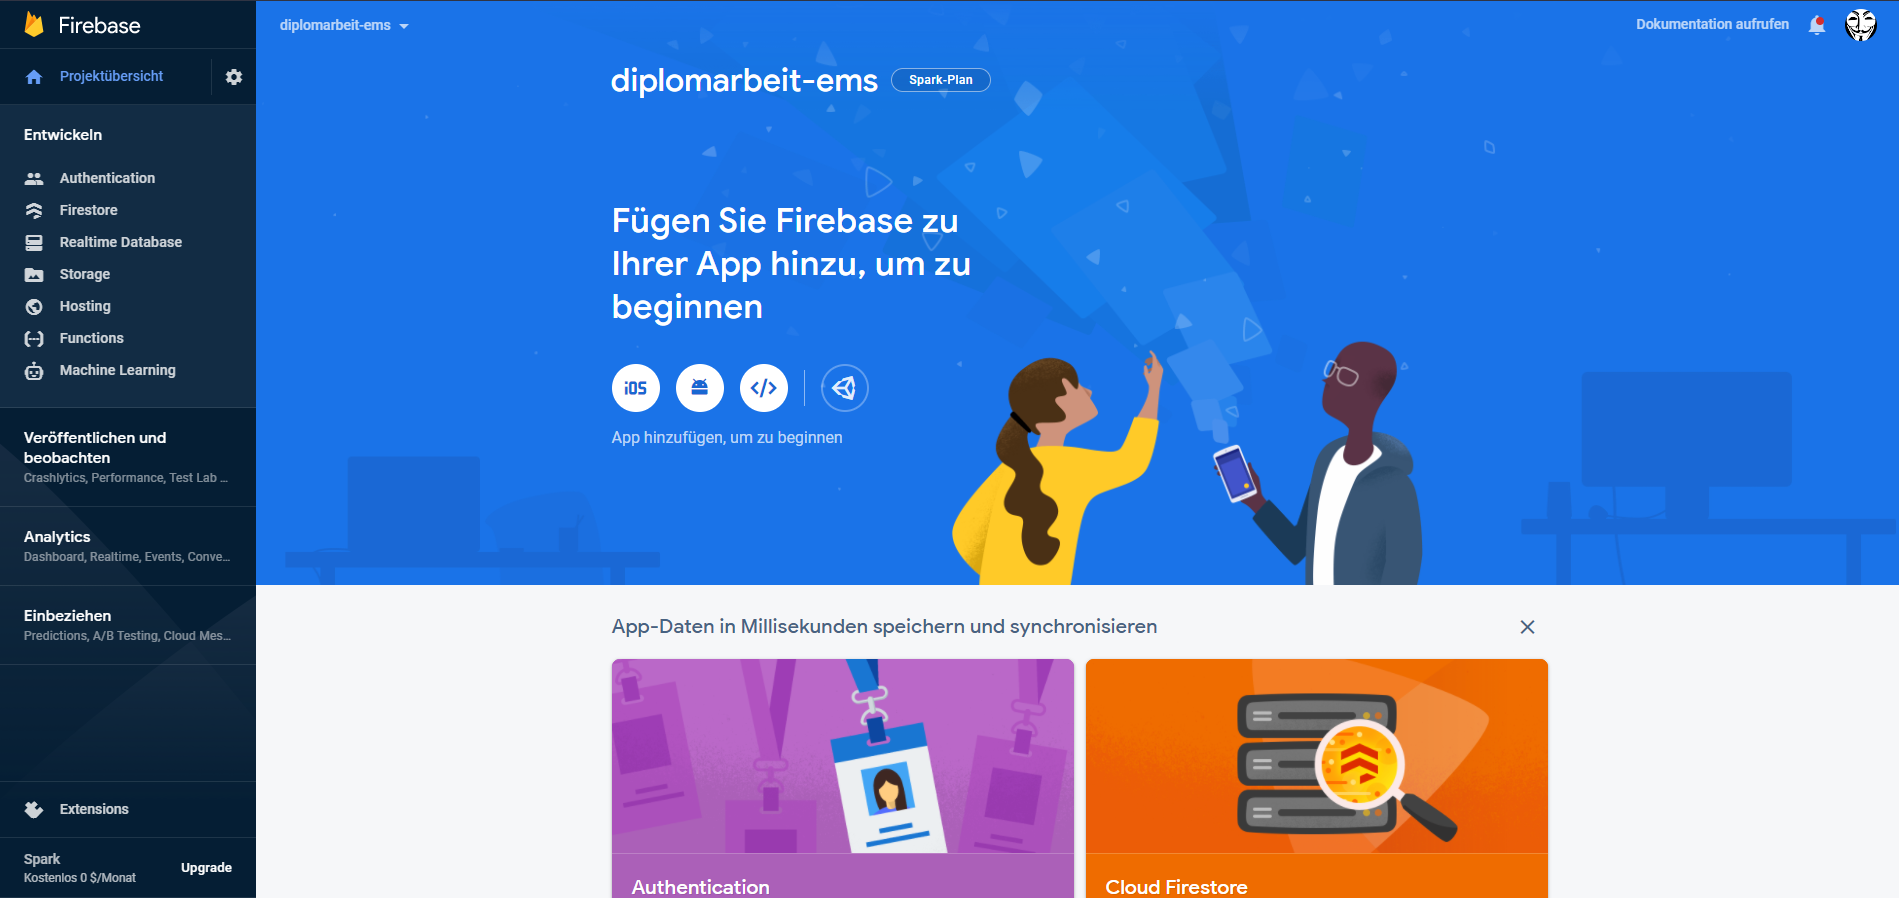
\includegraphics[width=\textwidth]{firebase-main.png}
        \caption{Datenbank erstellen}
    \end{figure}
\end{center}
Nachdem man auf der linken Seite auf \textbf{Realtime Database} geklickt hat, lädt die Hauptkomponente der Seite neu. Nun klickt man auf \textbf{Datenbank erstellen} (Abbildung 3.2).
\begin{center}
    \begin{figure}[H]
        \centering
        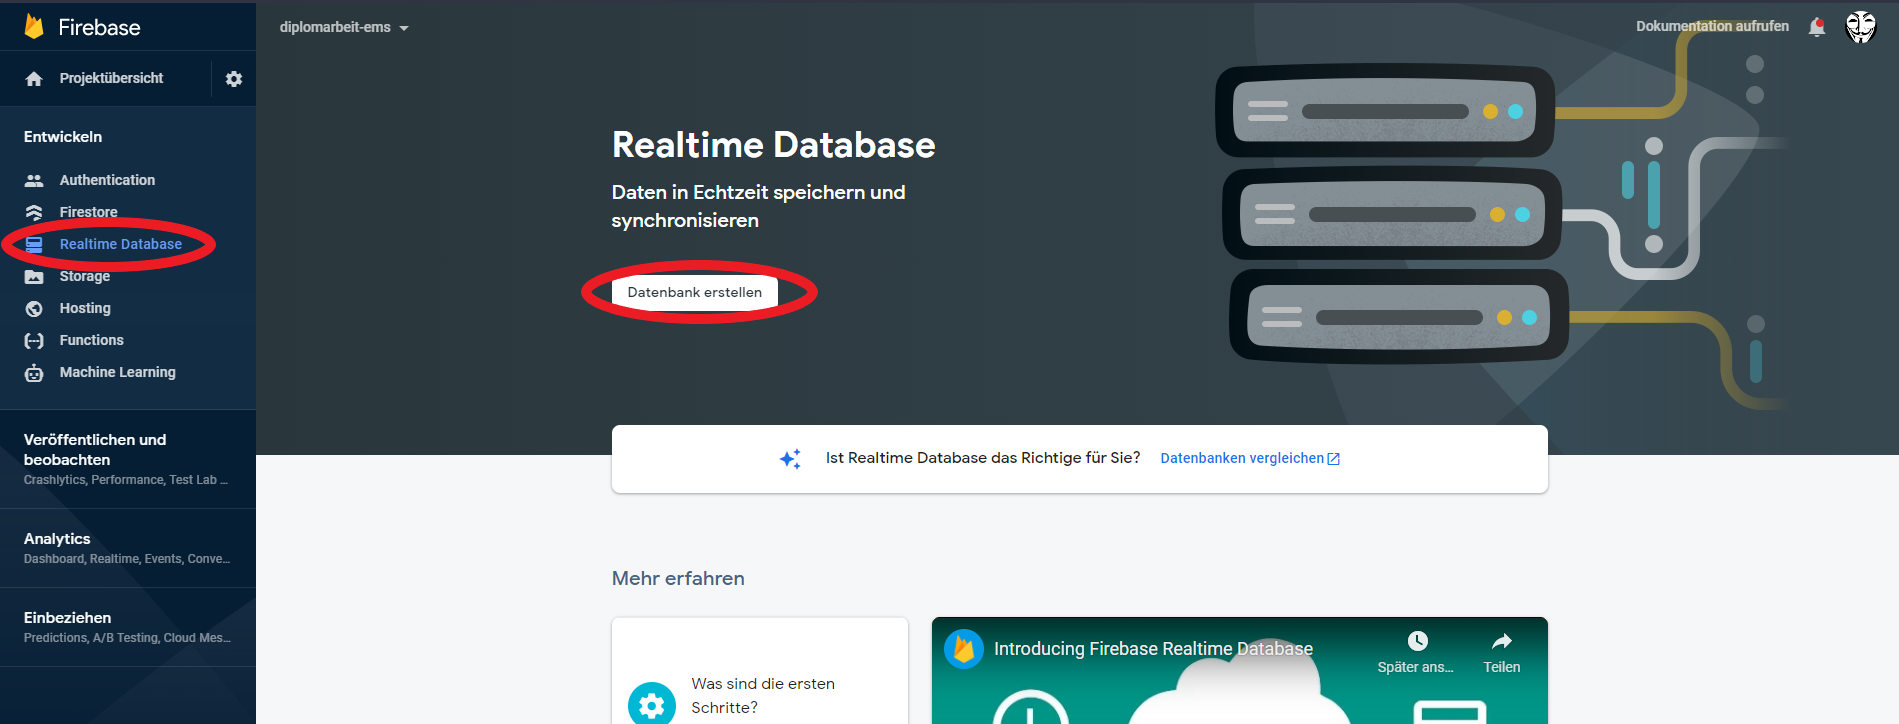
\includegraphics[width=\textwidth]{firebase-db1.png}
        \caption{Datenbank erstellen}
    \end{figure}
\end{center}
Danach erscheint ein Pop-up, in welchem man den physichen Ort, wo die Daten der Datenbank gespeichert werden, festlegt. Da die Software DSGVO konform sein muss, sollte ein Standort innerhalb der EU ausgewählt werden.
\begin{center}
    \begin{figure}[H]
        \centering
        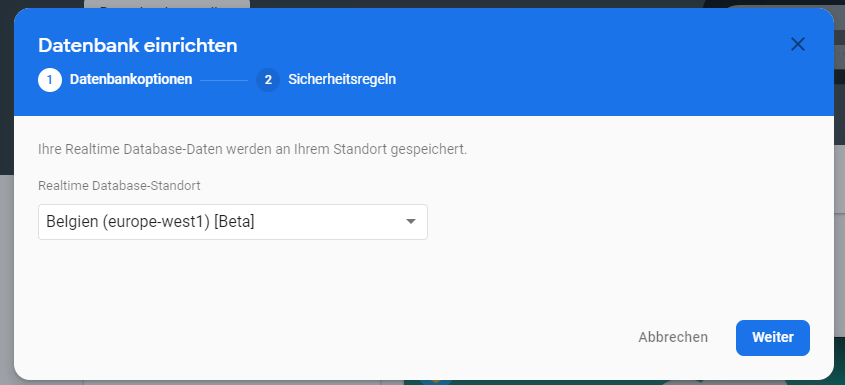
\includegraphics[width=\textwidth]{firebase-db2.png}
        \caption{Datenbank Standort}
    \end{figure}
\end{center}
Mit einem Klick auf \textbf{Weiter} gelangt man auf die zweite und letzte Seite des Pop-ups.
Hier kann man nun auswählen, ob die Datenbank direkt in Produktivbetrieb geht oder zuerst der Testmodus gestartet werden soll. Dies ist bei einer
noch aktiven Entwicklung zu empfehlen wie auf den Hinweisen in Abbildung 3.4 zu lesen ist.
\begin{center}
    \begin{figure}[H]
        \centering
        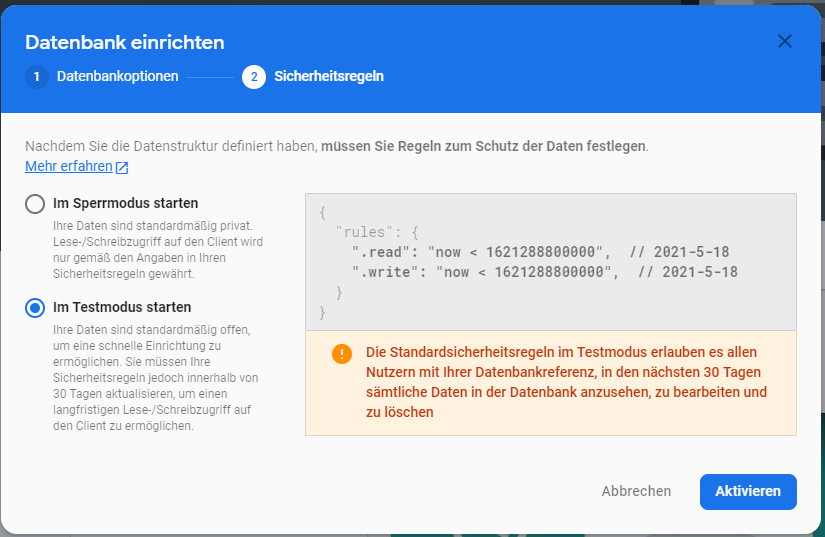
\includegraphics[width=\textwidth]{firebase-db3.png}
        \caption{Datenbank Modus}
    \end{figure}
\end{center}
Nun wurde eine fertige Realtime Database in Firebase erstellt. Damit die nachfolgende Angular App auch mit der Datenbank kommunizieren kann, müssen Lese- und Schreibrechte auf
jeden übertragen werden. Dies ist in Abbildung 3.5 zu sehen.
\begin{center}
    \begin{figure}[H]
        \centering
        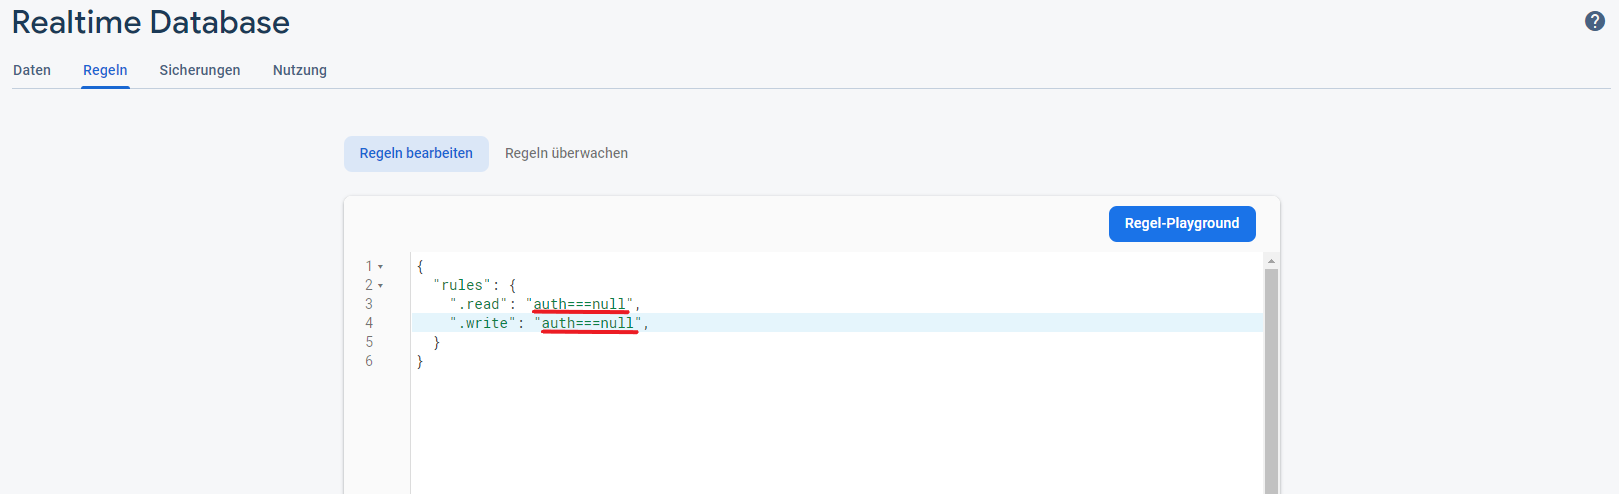
\includegraphics[width=\textwidth]{firebase-db4.png}
        \caption{Datenbank Regeln bearbeiten}
    \end{figure}
\end{center}
Dies war die Konfiguration der Datenbank hinter der Chatapplilation in der Firebase Cloud. Nun folgen eine Anleitung und einige Codesnippets zur Erstellung des eigentlich Chatprogrammes in Angular, welches später in das Hauptprogramm
EMS integriert wird.

Zuerst muss das Google Firebase SDK installiert und auch in einer neuen Angular App inkludiert werden. Bei der Angular Anwendung wurde routing aktiviert und CSS verwendet.
\begin{lstlisting}[language=bash]
    #Neue Angular App anlegen
    ng new [app-name]

    #Firebase Installieren
    npm install --save firebase

    #In Datei `src/app/app.component.ts` vom Home Verzeichnis 
    #des Projektes aus, Firebase importieren
    import firebase from "firebase/app"
\end{lstlisting}

Als nächstes wurden der API Key und die URL zur Datenbank in Firebase gesetzt. Den API Key findet man, indem man oben links auf die Projekteinstellungen geht, danach kommt eine Seite und es erscheint der Web-API-Schlüssel (Abb. 3.6).
\begin{center}
    \begin{figure}[H]
        \centering
        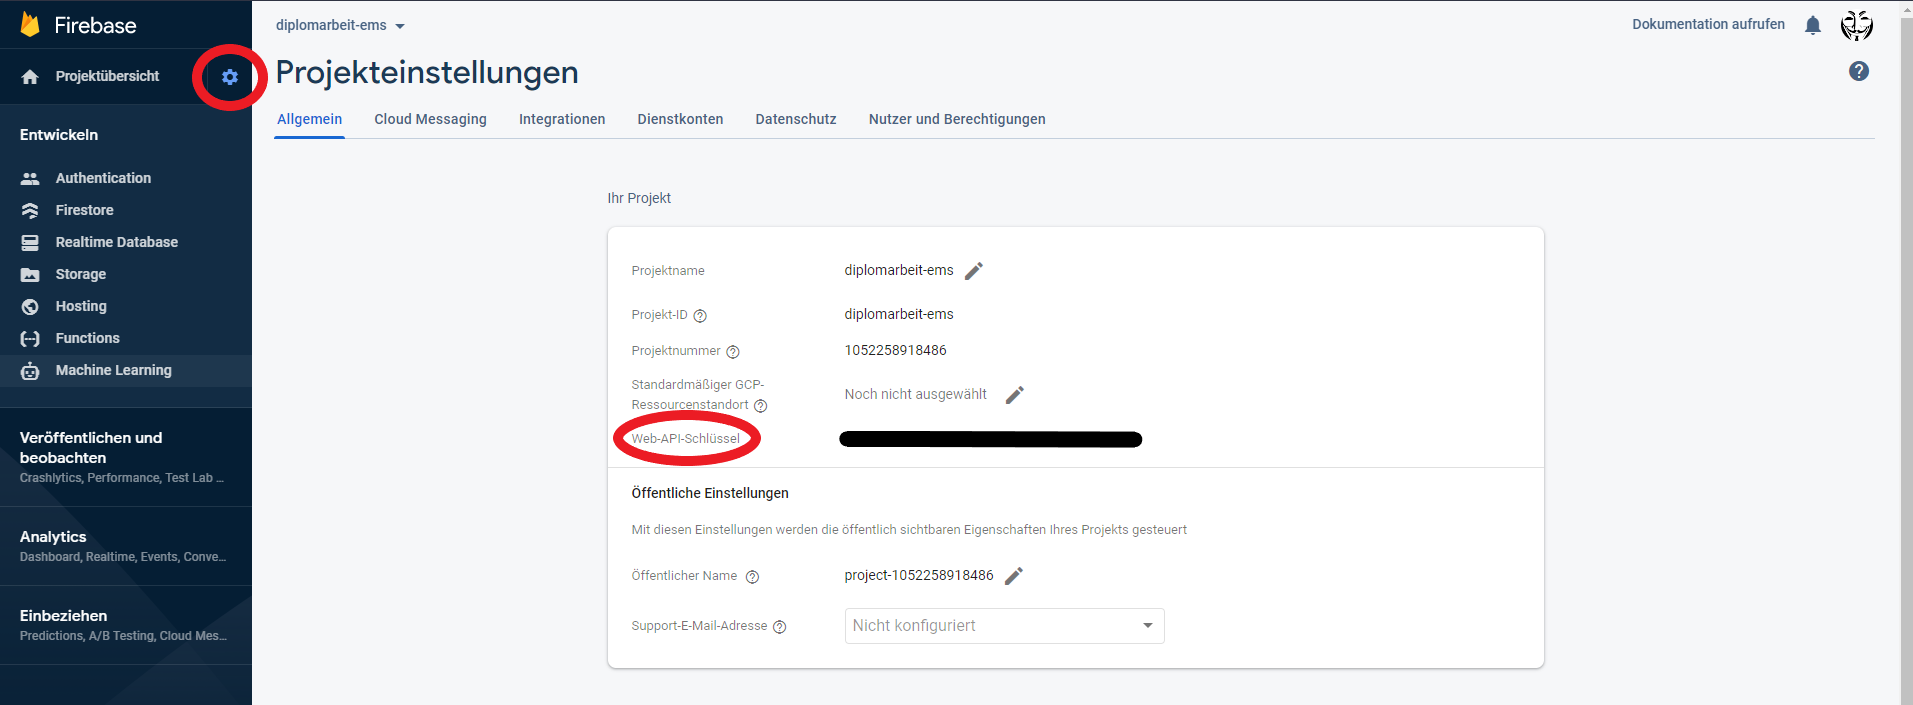
\includegraphics[width=\textwidth]{firebase-api.png}
        \caption{Firebase Web-API-Schlüssel}
    \end{figure}
\end{center}
Den Key und die URL müssen in einer Konstante im Code spezifiziert werden und die Firebase App im Konstruktor der Klasse AppComponent gestartet werden
\begin{lstlisting}[language=bash]
    #In Datei `src/app/app.component.ts` vom Home Verzeichnis als Konstante zu definieren
    const config = {
        apiKey: 'KEY',
        databaseURL: 'URL'
    };

    #Konstruktor anpassen
    constructor() {
        firebase.initializeApp(config);
    }
\end{lstlisting}
Das war der letzte Schritt bezüglich der Einstellungen von Firebase in Angular. Jetzt ist die Firebase Datenbank und das Angular Projekt fertig eingerichtet und es kann mit dem eigentlichen Entwickeln begonnen werden.

Im nachfolgenden Abschnitt werden nur die wichtigsten Codesnippets und Befehle der Firebase Chatapp gezeigt, da die Webapp später mit einem Patch in EMS inkludiert wird und dafür noch einige Anpassungen notwendig sind.
Zum Beispiel muss der Benutzer in EMS keinen Usernamen angeben, da er einen schon einen fixen Namen hat. Dieser wird dann automatisch aus der Datenbank ausgelesen. Weiters wurde in EMS Ionic benutzt, welches für die 
Kompatibilität auf den Mobilen Plattformen und das Design generell sorgt. In der Standalone Variante hier im Beispiel wurde nur Angular und HTML benutzt, daher sind Designs der Webapp nur temporär.
\subsection{Firebase Chatapp Implementierung}
Die Angular Webapp ist in vier Komponenten aufgeteilt. Im folgenden werden alle Komponenten in ihrer Grundfunktionalität beschrieben. Dies betrifft vor allem jeweils die Dateien mit den Endungen \textbf{*.component.ts}, da die 
HTML Dateien im weiteren Verlauf des Projektes und auch für das Verständnis der Chatfunktion obsolet sind.

Für die Darstellung der einzelnen Elemente der Standalone Webapplikation wurde Angular Materials\footcite{materials} wie in den Tutorials verwendet.
Diese Klasse mit ihren Komponent\footcite{matierials-componenten} wird jedoch in EMS nicht benötigt, da hier Ionic für die Darstellung verwendet wird.

Komponenten Namen:
\begin{itemize}
	\item addroom
	\item login
	\item chatroom
	\item roomlist
\end{itemize}
\textbf{login}: Die Komponente login wird in EMS später nicht mehr benötigt. Hier musste der Benutzer seinen Namen, welchen er in der Chatapp benutzen wollte, angeben. In EMS wird der Benutzername eines Promoters automatisch
auch in der Chatfunktion benutzt. Dieser kann nicht geändert werden, da auch alle Chats mit diesem Promoter verloren gehen würden.

\textbf{addroom}: Die Funktionalität in dieser Komponente liegt darin, einen neuen Chatraum anzulegen. In EMS integriert, wird diese Funktion nur einem Administratoren zu
Verfügung stehen. Ein Promoter wird automatisch immer einen einzigen Raum/Chat zu einem Administrator offen haben. Der Administrator kann später einen Raumnamen angeben und ein Event auswählen. Dann kann er zu diesem Raum Personen,
welche dem Event zugeteilt sind, auswählen und zu chatten beginnen.

Folgende Variablen sind in der Klasse von addroom angegeben:
\begin{lstlisting}[language=bash]
    roomForm: FormGroup;
    username = '';
    roomname = '';
    ref = firebase.database().ref('rooms/');
\end{lstlisting}
Falls ein neuer Raum hinzugefügt wird, wird in der Firebase Datenbank überprüft, ob bereits ein Raum mit der gleichen Bezeichnung wie vom Benutzer angegeben existiert. Falls ja, wird eine entsprechende Fehlermeldung ausgegeben. Falls
nicht, wird wie im nachstehenden Codesnippet zu sehen ist, ein neuer Raum erstellt und in die Firebase Datenbank eingefügt. Danach wird der Benutzer zu der Komponente \textbf{roomlist} geroutet.
\begin{lstlisting}[language=bash]
    #Erstellen eines neuen Raumes und einfuegen in Firebase
    const newRoom = firebase.database().ref('rooms/').push();
    newRoom.set(room);

    #routing zurueck zur Chatraum Uebersicht
    this.router.navigate(['/roomlist']);
\end{lstlisting}
\textbf{roomlist}: Diese Komponente zeigt alle momentan verfügbaren Chaträume an. Die Daten werden im Konstruktor der roomlist Klasse geladen.

Eine Funktion, \textbf{enterChatroom(string roomname)}, wird bei Auswahl eines Raumes ausgeführt. Es wird eine Konstante namens \textbf{chat} erstellt. Diese Variable wird für den Zutritt zu einem Chatraum benötig, da sie 
Infomationen wie Name und Datum des betretens des Raumes enthält. Weiters wird in dieser Funktion der neue Benutzer zu dem \textbf{roomusers} Dokument in der Firebase Datenbank hinzugefügt.

\begin{lstlisting}[language=bash]
    #Konstante
    const chat = { roomname: '', username: '', message: '', date: '', type: '' };

    #Speichern bei fertig gesetzter Konstante in Firebase
    const newMessage = firebase.database().ref('chats/').push();
    newMessage.set(chat);

    firebase.database().ref('roomusers/').orderByChild('roomname').equalTo(roomname).on('value', (resp: any) => {
        let roomuser = [];
        roomuser = snapshotToArray(resp);
        const user = roomuser.find(x => x.username === this.username);
        #if Benutzer in File, dann als online anzeigen
        #else (Benutzer nicht im File) in Firebase Datenbank pushen und als online anzeigen
    .});
\end{lstlisting}

Danach wird der Benutzer weiter zu der Komponente \textbf{chatroom} geroutet.

\textbf{chatroom}: Zuletzt die wichtigeste Komponente. Hier ist der eigentliche Chat und dessen Funktionalität implementiert. Beim Erstellen der Komponente und Laden der Klasse wird zuerst eine Komponente zum Konvertieren
des Firebase responses definiert.

\begin{lstlisting}[language=bash]
    export const snapshotToArray = (snapshot: any) => {
    const returnArr = [];

    snapshot.forEach((childSnapshot: any) => {
        const item = childSnapshot.val();
        item.key = childSnapshot.key;
        returnArr.push(item);
    });

    return returnArr;
};
\end{lstlisting}

Die Variablen in der Chatroom-Klasse sehen folgendermaßen aus:

\begin{lstlisting}[language=bash]
    #Autoscrooling fuer den Chat bei Nachrichtenerhalt
    @ViewChild('chatcontent') chatcontent: ElementRef;
    scrolltop: number = null;
  
    #Variablen mit Nachrichten, Benutzername und Nutzer im Chatraum
    chatForm: FormGroup;
    nickname = '';
    roomname = '';
    message = '';
    users = [];
    chats = [];
\end{lstlisting}

Die Daten der Variablen werden im Konstruktor gesetzt. Dieser geht über mehrer Zeilen, daher wird nur ein wichtiger Ausschnitt gezeigt.

\begin{lstlisting}[language=bash]
    #Setzen des Arrays, welche alle Chatnachrichten beinhaltet mithilfe der snapshot Konstante
    firebase.database().ref('chats/').on('value', resp => {
        this.chats = [];
        this.chats = snapshotToArray(resp);
        setTimeout(() => this.scrolltop = this.chatcontent.nativeElement.scrollHeight, 500);
    });
    
    #Setzen der des Userarrays, welche alle Teilnehmer des Chatraumes angibt
    firebase.database().ref('roomusers/').orderByChild('roomname').equalTo(this.roomname).on('value', (resp2: any) => {
        const roomusers = snapshotToArray(resp2);
        this.users = roomusers.filter(x => x.status === 'online');
    });
\end{lstlisting}

Wenn ein User im Chatraum eine Nachricht absendet, wird die Funktion, \textbf{onFormSubmit(any Form)}, aufgerufen.
Hier wird eine \textbf{chat} Konstante wie schon in der roomlist Komponente erstellt und mit den entsprechenden Daten befüllt. Diese Konstante wird an die Firebase Datenbank gesendet und die chatForm
wird wieder freigegeben.

\begin{lstlisting}[language=bash]
onFormSubmit(form: any) {
    const chat = form;
    chat.roomname = this.roomname;
    chat.nickname = this.nickname;
    chat.date = this.datepipe.transform(new Date(), 'dd/MM/yyyy HH:mm:ss');
    chat.type = 'message';

    const newMessage = firebase.database().ref('chats/').push();
    newMessage.set(chat);
    
    this.chatForm = this.formBuilder.group({
      'message' : [null, Validators.required]
    });
 }
\end{lstlisting}
\newpage